% !TEX root = ../eval.tex

\section{Methods}%
\label{sec:data}

\subsection{Dataset}%
\label{sub:dataset}

\begin{itemize}

    \item Money Dashboard can access up to three years of historic data for
        each account a user links to their account.

    \item Each user for whom we have sufficient data thus serves as both a
        treatment unit and a potential control unit.

    \item Limitations: We have more data for users that signed up later. So average user in
        the study is not the average MDB user. If time of signup is mainly
        driven by financial savyness, then study sample is closer to overall
        population than MDB sample (if we rank groups as early joiners > late
        joiners > never joiners in terms of financial sophistication). If,
        however, signup reflects something like openness to newness, then it's
        not necessarily correlated with financial savyness. Either way, we
        might ignore it for now. We could test whether behaviour differs
        between early or late adopters, but that doesn't seem important enough.

\end{itemize}

\subsection{Data preprocessing}%
\label{sub:data_preprocessing}

\paragraph{Cleaning}%
\label{par:cleaning}

MDB cleaning (mdb/mdb/clean.py)
\begin{itemize}
    \item About 75 percent of transactions are not automatically categorised,
        and we drop transactions that have no automatic tag. Dropping untagged
        transactions means that we might underestimate spending and savings,
        but entures that we do not miscategorise transactions.

    \item Custom tag classifications.

    \item Drop transactions for which user ID, account ID, date, amount, and
        transaction description are identical. This will drop some genuine
        transactions, such as someone buying two identical cups of coffees at
        the same coffee shop on the same day. However, data inspection suggests
        that in most cases, we remove genuine duplicates.
\end{itemize}


\paragraph{Sample selection}%
\label{par:sample_selection}

We select our sample so as to include users for whom we can be reasonably
certain that we observe all relevant financial transactions, and do so for at
least six months before and after they sign up to the app. In addition to that,
we exclude users who might use the app for business purposes as well as
pensioneers, whose financial objectives might be different.

\begin{table}
\centering
\caption{Sample selection}\label{tab:selection}
\begin{tabular}{lrrrr}
\toprule
                                       &  Users & User-months &       Txns & Txns (m\pounds) \\
\midrule
                            Raw sample & 27,175 &     795,338 & 65,972,558 &          12,527 \\
             Drop first and last month & 26,565 &     741,170 & 64,157,932 &          12,179 \\
  At least 6 months of pre-signup data & 11,835 &     310,517 & 29,244,871 &           5,743 \\
 At least 6 months of post-signup data &  6,404 &     195,050 & 19,681,242 &           3,957 \\
          At least one current account &  5,833 &     178,845 & 18,257,300 &           3,738 \\
          At least one savings account &  4,506 &     138,181 & 14,485,916 &           3,133 \\
At least \pounds5,000 of annual income &  1,877 &      57,064 &  6,493,155 &           1,386 \\
           At least 10 txns each month &  1,686 &      51,190 &  5,935,336 &           1,262 \\
  At least \pounds200 of monthly spend &  1,478 &      44,641 &  5,333,532 &           1,135 \\
      Complete demographic information &  1,240 &      38,087 &  4,598,590 &             952 \\
                           Working age &  1,219 &      37,377 &  4,529,599 &             929 \\
                          Final sample &  1,219 &      37,377 &  4,529,599 &             929 \\
\bottomrule
\end{tabular}

\tabnote{\textwidth}{Number of users, user-months, transactions, and
transaction volume in millions of British Pounds left in our sample after each sample selection step. Link to sample selection
code:
\href{https://github.com/fabiangunzinger/mdb_eval/blob/main/src/data/selectors.py}{\faGithub}.}
\end{table}


Table~\ref{tab:selection} lists the precise conditions we applied to implement
these criteria and their effect on sample size. We remove the first and last
month of data for all users because we are unlikely to observe all transactions
for these months. We also drop test users, since their objectives for app use
might have been different from ordinary users.\footnote{We cannot identify test
users precisely, but drop users who signed up prior to or during the first year
the app was in operation.}

To ensure that we observe users for at least 12 months around app signup, we
require 6 months of data before the signup month, and another five months after
the signup month. Our main outcome variable is netflows into a user's savings
accounts. It is thus critical that we observe enough historical data for these
savings accounts to ensure that we observe all transactions during our 12 month
perdiod of interest. This is complicated by the fact that we cannot see when an
account was opened at the bank, but only when it was added to the app. While
cases where a user adds an account to the app as soon as it was opened are
unproblematic, users will often add accounts after they were opened, either
because they have accounts that they opened before signing up to the app, or
because they opened new accounts after signup but add them to the app with a
delay. In such cases, it is critical that, once the account is added, we
observe the complete historical data up to 6 months before signup or up to the
month in which the account was opened, whichever happened later. To see why
this is critical, imagine a scenario where a user opens an account 10 months
before they sign up to the app, makes a monthly transfter to the account of
\pounds100, adds the account to the app on signup, but we onserve only 3 months
of historical data. In this case we would observe that the user saved
\pounds300 before signup and \pounds600 after, and erroneously conclude that
post signup savings were twice as high. The most extreme case we need to cover
is that of a user opening a savings account more than six months before signup
and adding the account to the app five months after signup, in which case we
need to be sure to observe 12 months of historical data. As shown in
Appendix~\ref{app:data}, all major banks started providing 12 months of
historical data for current and savings accounts from April 2017 onwards, which
is why we restrict our sample to users who signed up in or after that month.

To ensure that we can be reasonably certain to observe users have added all
their financial accounts to the app, we restrict our sample to users with at
least one savings and current account, with an annual income of at least
\pounds5,000, and a minimum of 10 transactions and a spend of \pounds200 every
month. To remove users who might use the app for business purposes, we drop
users with more than 10 active accounts in any given month. Finally, we remove
users for whom we cannot observe all demographic information we use as
covariates in our analysis, and users who are not between the ages of 18 and
65, as their financial objectives are plausibly different.


\paragraph{Data transformations:}%
\label{par:data_transformations}

To minimise the influence of outliers, we winsorise spend, income, and savings
accounts flow variables at the 1 percent level or -- if we winsorise on both
ends of the distribution -- at the 0.5 percent level.


\subsection{Summary statistics}%
\label{sub:summary_statistics}

Figure~\ref{fig:sample_description} describes the sample.

\begin{figure}[H]
    \centering
    \caption{Sample characteristics}
    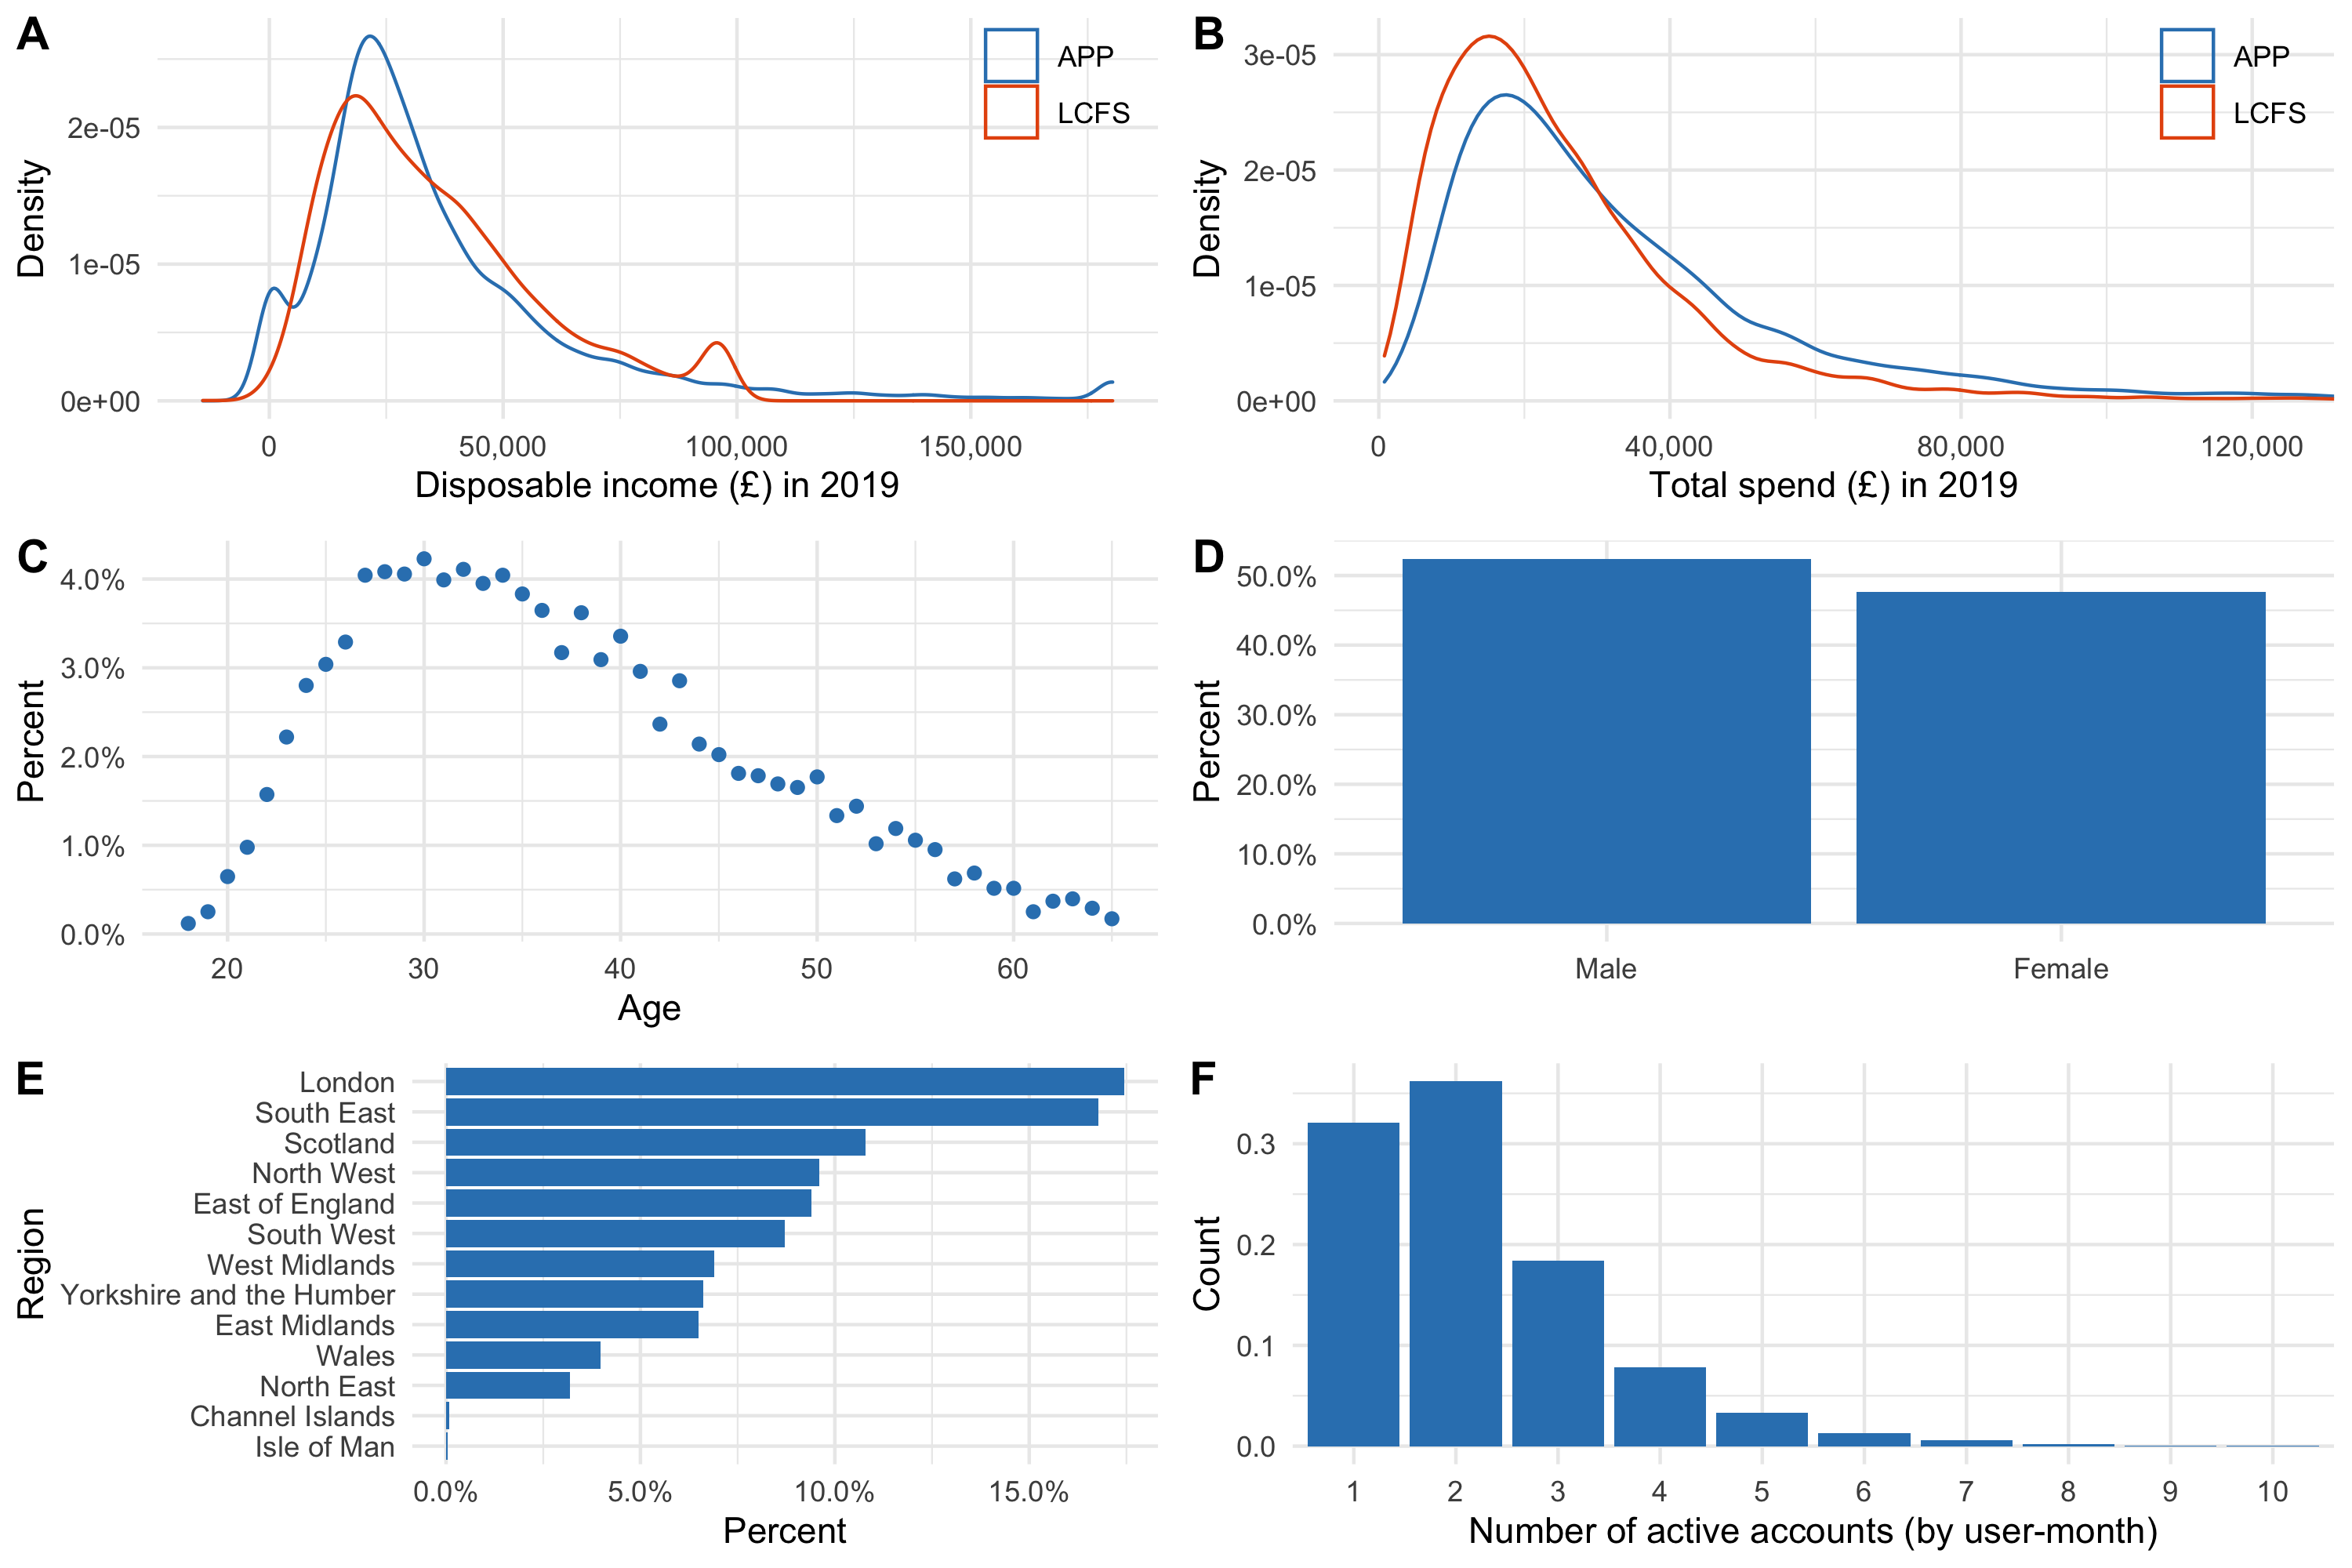
\includegraphics[width=\linewidth]{\figdir/sample_description.png}
    \label{fig:sample_description}
    \fignote{\textwidth}{Panels A and B show the distribution of disposable
        income and total spending in 2019, respectively, benchmarked against
        the 2018/19 wave of the ONS Living Cost and Food Survey (LCFS). The
        remaining panels show the data distributions of age, gender, region,
    and the number of active accounts.}%
\end{figure}

Table~\ref{tab:sumstats} provides summary statistics.


\begin{table}[htbp]
   \centering
   \tiny
   \begin{threeparttable}[b]
      \caption{\label{tab:reg_compare} Regression results}
      \begin{tabular}{lcccccc}
         \tabularnewline \midrule \midrule
         Dependent Variable: & \multicolumn{6}{c}{Net-inflows}\\
         Model:                     & (1)                   & (2)                & (3)                & (4)                & (5)               & (6)\\  
         \midrule
         \emph{Variables}\\
         App use                    & 14.330$^{**}$         & 15.303$^{***}$     & 15.303$^{***}$     & 19.381$^{***}$     & 15.963$^{**}$     & 20.207$^{***}$\\   
                                    & [2.650; 26.009]       & [3.686; 26.919]    & [3.686; 26.919]    & [7.110; 31.652]    & [1.881; 30.045]   & [7.940; 32.473]\\   
         Month income               &                       & 0.053$^{***}$      & 0.053$^{***}$      & 0.060$^{***}$      & 0.053$^{***}$     & 0.058$^{***}$\\   
                                    &                       & [0.049; 0.058]     & [0.049; 0.058]     & [0.045; 0.075]     & [0.045; 0.060]    & [0.043; 0.073]\\   
         Month spend                &                       & -0.077$^{***}$     & -0.077$^{***}$     & -0.100$^{***}$     & -0.076$^{***}$    & -0.098$^{***}$\\   
                                    &                       & [-0.081; -0.073]   & [-0.081; -0.073]   & [-0.109; -0.091]   & [-0.091; -0.061]  & [-0.107; -0.089]\\   
         Disc. spend                &                       & 138.940$^{***}$    & 138.940$^{***}$    & 169.002$^{***}$    & 132.862$^{***}$   & 156.441$^{***}$\\   
                                    &                       & [115.597; 162.282] & [115.597; 162.282] & [128.874; 209.129] & [90.975; 174.750] & [115.907; 196.976]\\   
         Female                     &                       & -14.521$^{***}$    & -14.521$^{***}$    &                    & -14.247$^{***}$   &   \\   
                                    &                       & [-24.998; -4.044]  & [-24.998; -4.044]  &                    & [-21.206; -7.289] &   \\   
         Generation $=$ GenX        &                       & 39.071$^{***}$     & 39.071$^{***}$     &                    & 39.379$^{**}$     &   \\   
                                    &                       & [19.258; 58.885]   & [19.258; 58.885]   &                    & [9.611; 69.148]   &   \\   
         Generation $=$ Millennials &                       & 71.330$^{***}$     & 71.330$^{***}$     &                    & 71.699$^{***}$    &   \\   
                                    &                       & [51.964; 90.697]   & [51.964; 90.697]   &                    & [40.338; 103.060] &   \\   
         Generation $=$ GenZ        &                       & 42.302             & 42.302             &                    & 43.095$^{*}$      &   \\   
                                    &                       & [-9.381; 93.985]   & [-9.381; 93.985]   &                    & [-7.002; 93.192]  &   \\   
         Intercept                  & -20.523$^{***}$       & -59.208$^{***}$    & -59.208$^{***}$    &                    &                   &   \\   
                                    & [-30.679; -10.368]    & [-84.179; -34.237] & [-84.179; -34.237] &                    &                   &   \\   
         \midrule
         \emph{Fixed-effects}\\
         User FE                    &                       &                    &                    & Yes                &                   & Yes\\  
         Month FE                   &                       &                    &                    &                    & Yes               & Yes\\  
         \midrule
         \emph{Fit statistics}\\
         Observations               & 184,847               & 184,847            & 184,847            & 184,847            & 184,847           & 184,847\\  
         R$^2$                      & $3.13\times 10^{-5}$  & 0.01132            & 0.01132            & 0.10137            & 0.01203           & 0.10203\\  
         Within R$^2$               &                       &                    &                    & 0.00905            & 0.01117           & 0.00885\\  
         \midrule \midrule
         \multicolumn{7}{l}{\emph{Signif. Codes: ***: 0.01, **: 0.05, *: 0.1}}\\
      \end{tabular}
   \end{threeparttable}
\end{table}




We use data from the 2018-2019 wave of the Office of National Statistics' Living Costs and Food
Survey (LCFS).\footnote{We accessed the data via the UK Data Service at the
following url:
\url{https://beta.ukdataservice.ac.uk/datacatalogue/studies/study?id=8686}.}
Data covers the period between April 2018 and March 2019.



\subsection{Treatment}%
\label{sub:treatment}

A user changes treatment status from untreated to treated when they start using
the app. Figure~\ref{fig:treatplot_sample_raw} shows the treatment history for
200 randomly selected users.

\begin{figure}[H]
    \centering
    \caption{Treatment assignment plot}%
    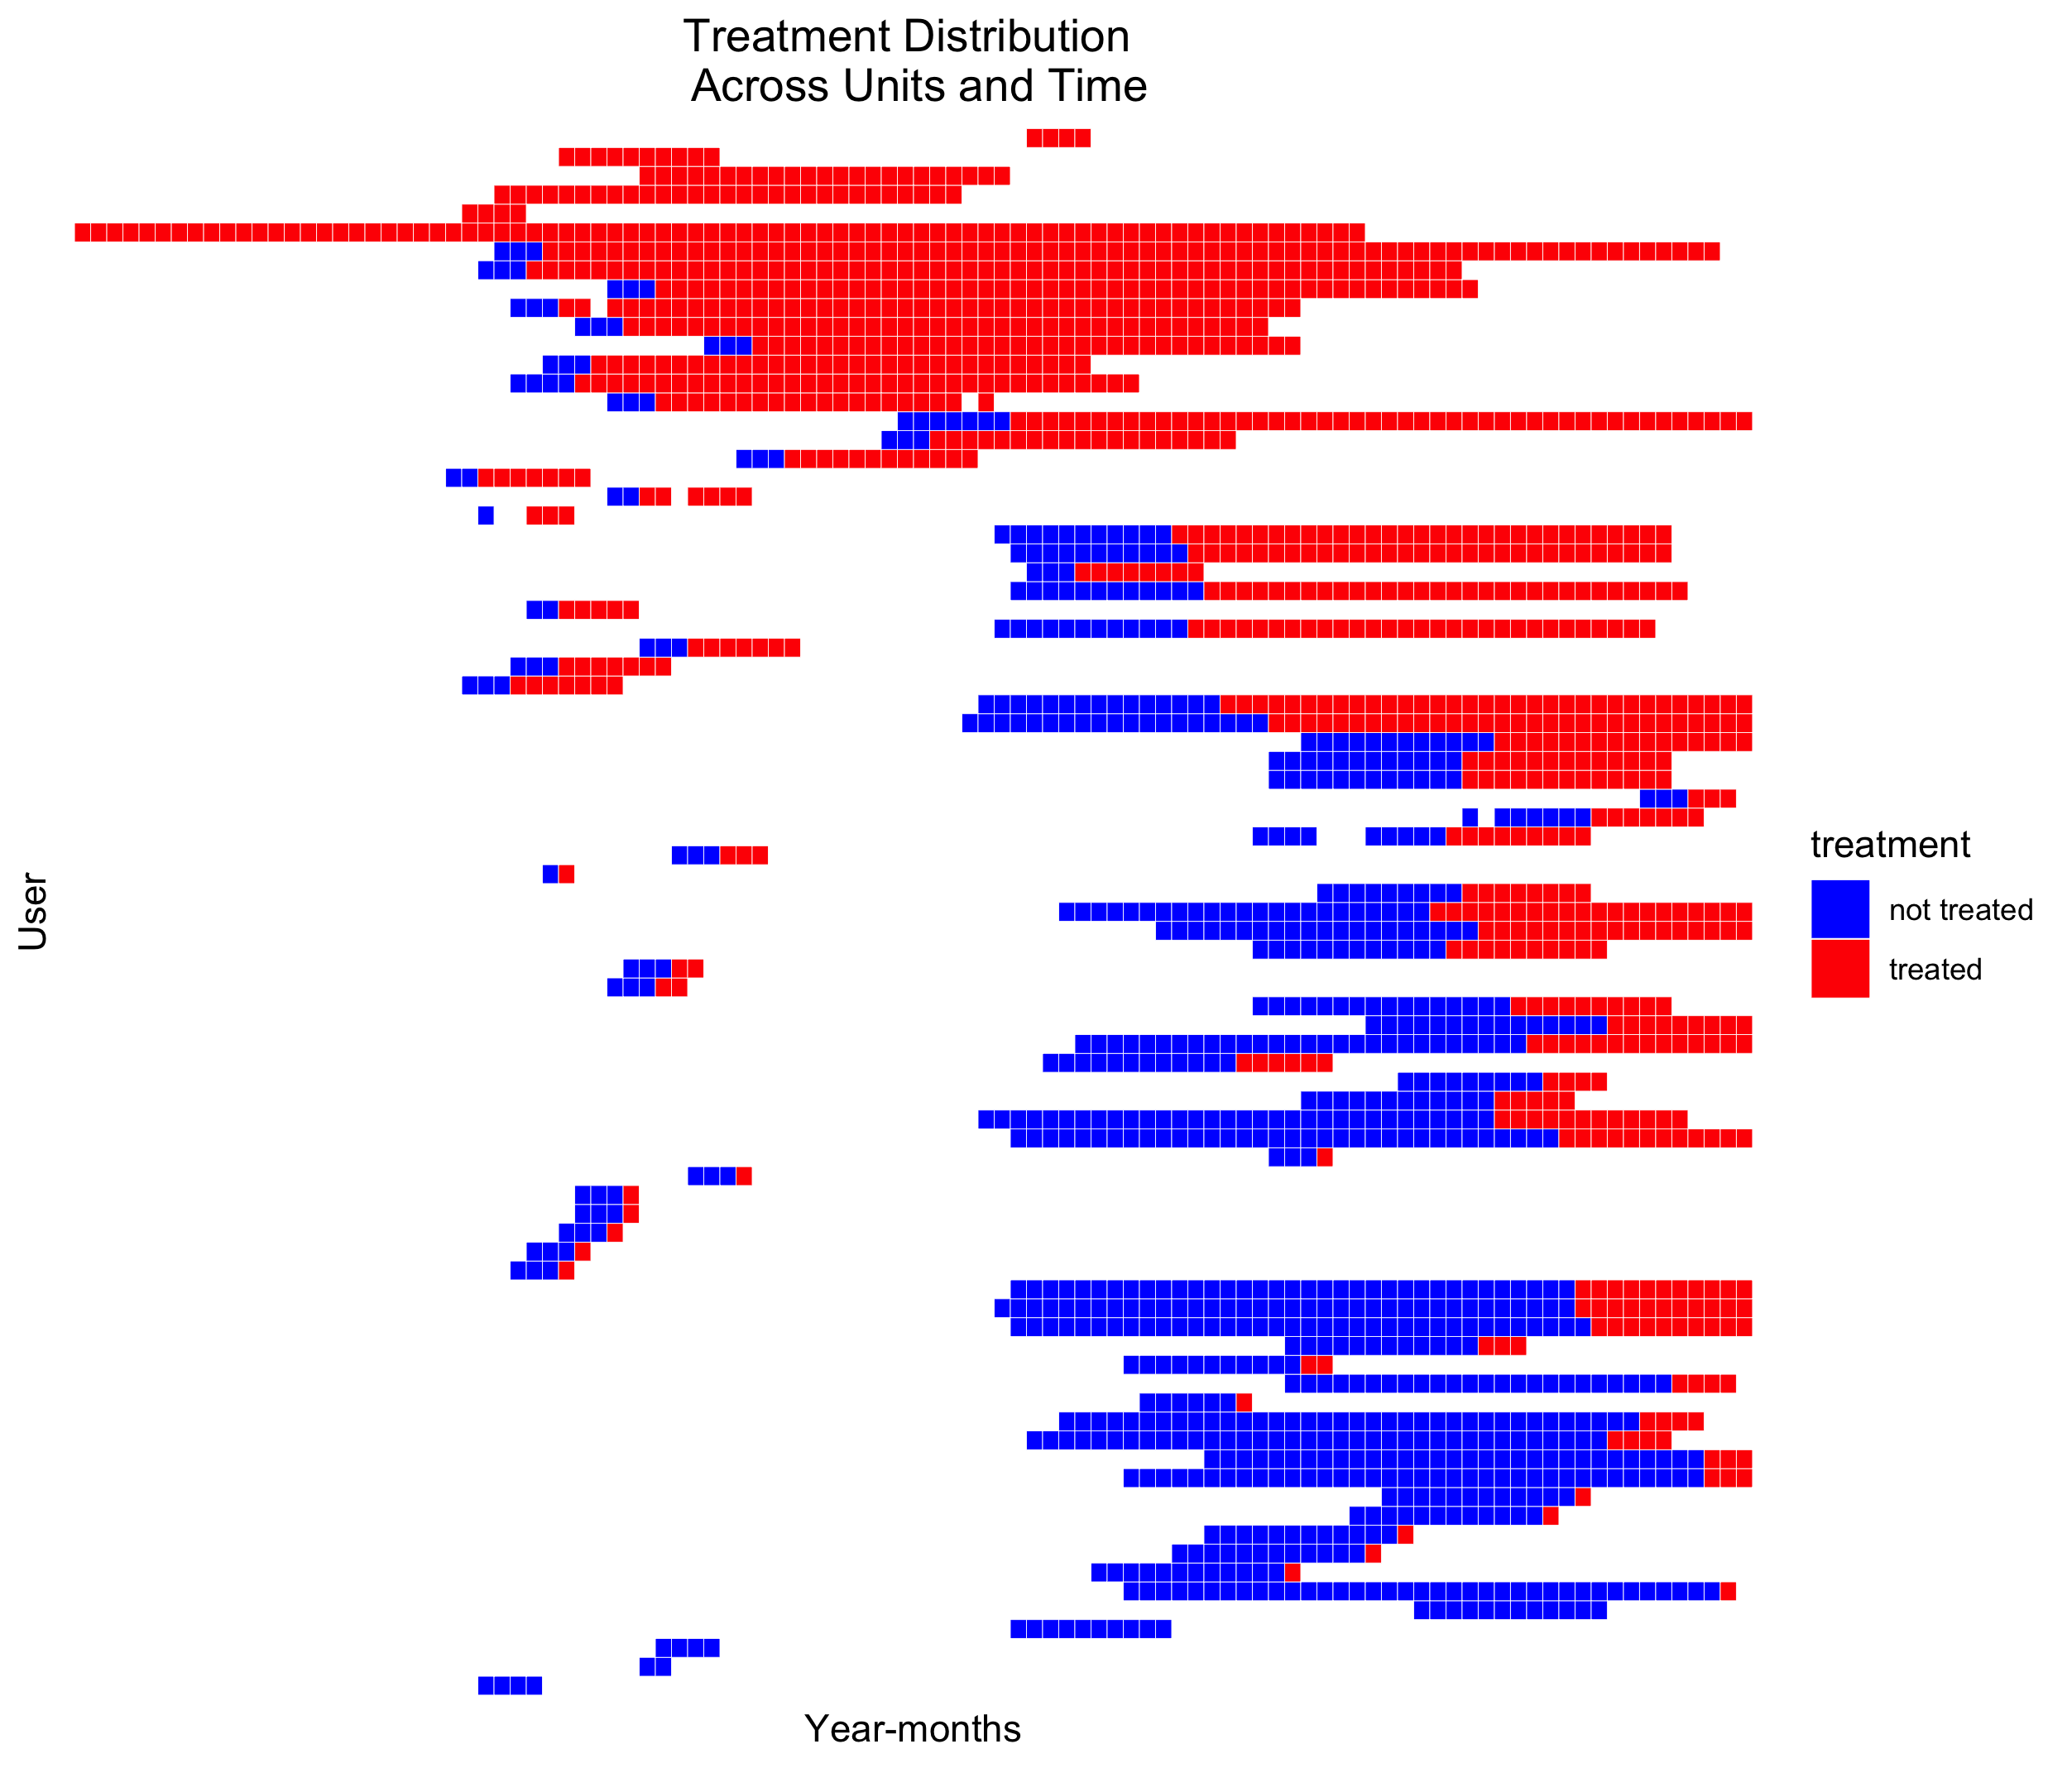
\includegraphics[width=0.8\linewidth]{\figdir/treatplot_sample_raw.png}
    \label{fig:treatplot_sample_raw}

    \fignote{\textwidth}{Each horizontal line shows the observed pre and post
        signup periods in blue and red, respectively, for one of 200 randomly
        selected users. The faint vertical white lines indicate month borders,
        whitespace indicates periods in which we do not observe the user. To
    the left of the observed period, this is because the app cannot access data
before that point when the user signs up; to the right, because they have
stopped using the app.}

\end{figure}


\subsection{Outcomes}%
\label{sub:outcomes}

Savings... see Table~\ref{tab:vars} for details.

For a more nuanced understanding of how app use affects savings we also
consider net-savings -- total savings account inflows minus outflows -- as a
proportion of monthly income to see whether a willingness to save more might be
offset by a (later) need to withdraw funds, and a dummy variable for whether a
user has any savings account inflows in a given month to see whether the app
helps users save at all. To investigate possible channels, we consider total
spend, highly discretionary spend, banking charges, the total amount of
borrowing, as well as payday borrowing, all as proportion of monthly income.



Net savings (\textit{netflows\_norm})
Inflows into minus outflows out of all of a user's savings accounts divided
by monthly income. To capture only ``user-generated'' flows, we exclude
interest and ``save the change'' transactions, as well as transactions of
less than \pounds5 in absolute
value. Monthly income and raw inflows and outflows are winsorised at the 1
percent level.
We focus on net inflows to capture effective savings.

Positive net savings dummy (\textit{has\_pos\_netflows})
Dummy equal to 1 if there were positive net savings (as defined above).
Captures extensive margin of savings (change in number of months with positive
net deposits)

Positive net savings (\textit{pos\_netflows})
Equal to net savings if there were positive net savings.
Captures intensive margin of savings (change in deposit amount in months with
positive net deposits)

\begin{figure}[H]
    \centering
    \caption{Savings patterns}%
    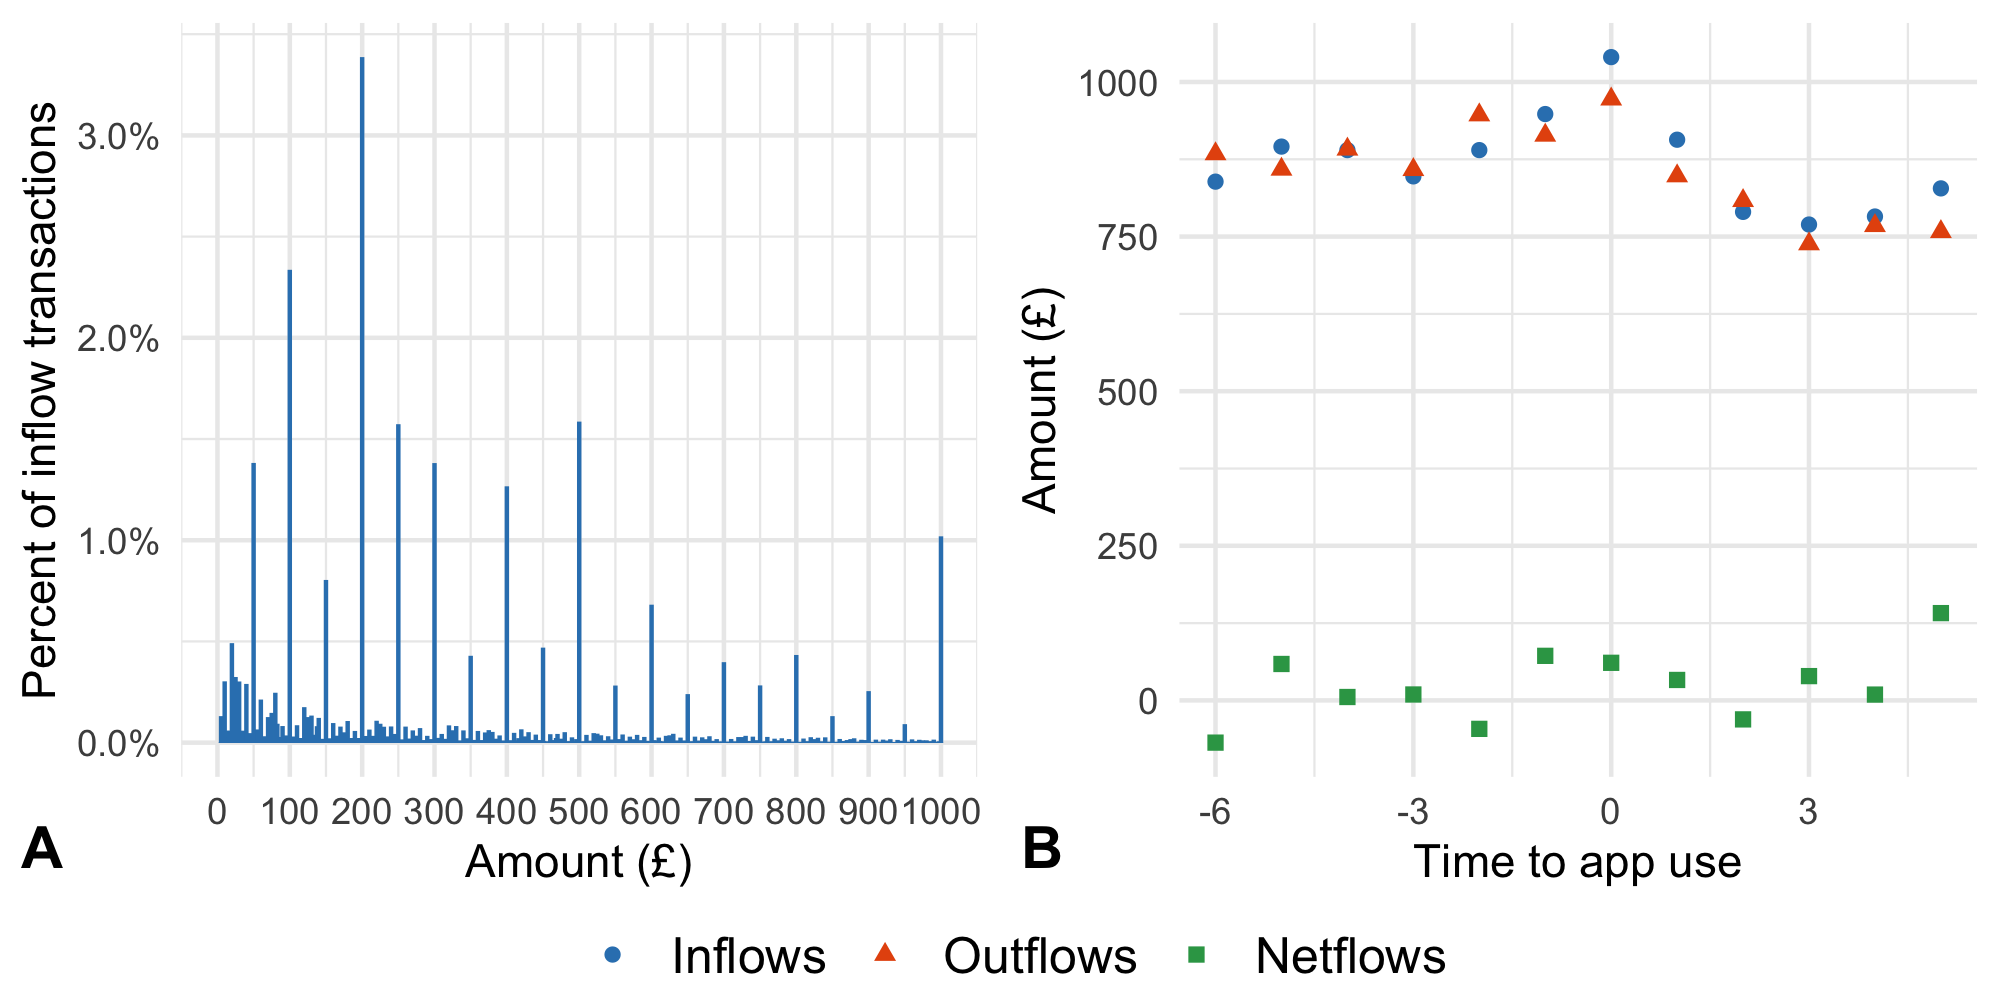
\includegraphics[width=\linewidth]{\figdir/savings_patterns.png}
    \label{fig:\figdir/savings_patterns}
    \fignote{\textwidth}{Panel A shows distribution of savings account inflow
        amounts, making clear that most transactions are the kinds of round
        amounts we would expect savings transactions to be. The data is
        truncated at \pounds1000. Panel B hows inflows, outflows, and netflows
        into savings accounts for six months before and five months after app
    use.}

\end{figure}


\paragraph{Adjusting for multiple hypothesis tests}%
\label{par:adjusting_for_multiple_hypothesis_tests}
We think of our secondary outcomes as exploratory and do not make any
adjustments for multiple hypothesis testing.\footnote{For a recent
game-theoretically motivated discussion of when and how to correct for multiple
hypothesis testing, see \citet{viviano2021should}.} An alternative approach,
based on \citet{anderson2008multiple}, would be to group outcomes into
``savings'', ``spending'', ``borrowing'', and ``fees'', and consider them as
different dimensions of a latent variable of interest which we might call
``financial management skills''. We do not do that for two reasons: first and
foremost, because we think it is natural to think of the amount saved as the
ultimate outcome and of other outcomes as providing a more nuanced
understanding of savings behaviour or as suggesting possible channels through
which app use affects savings. Thinking of savings as the main goal is also
reflected in Money Dashboard's main promise, which is to help users spend less
and save more, as shown in Figure~\ref{fig:mdb_website}. Second, as pointed out
in \citet{carlin2017fintech}, incurring overdraft fees is not an unambiguous
sign of a financial mistake, as the opportunity to go into overdraft confers a
benefit to the consumer.\footnote{For further discussions on fees, see
\citet{jorring2020financial, stango2009consumers}.}


\subsection{Covariates}%
\label{sub:covariates}

We control for baseline behaviour, events, and personal characteristics that,
to various degrees, capture a person's need, capacity, motivation, and
awareness to save. Table~\ref{tab:vars} lists all covariates used
together with their definition and the rationale for including them. For all
variables, we include contemporaneous values as well as lags for up to 6
periods. In addition, we control for the previous six months of savings to
capture time-invariant unobserved drivers of savings behaviour (in
specifications without fixed effects) as well as a possible signal for a higher
or lower need for future savings.

Following \citet{vanderweele2019principles} we include covariates that affect
either outcomes or the propensity for treatment or both, exclude from this
set of variables those that are instruments (affect the outcome only through their effect on
treatment propensity) and add to it proxies for unobserved variables that are a
common cause of both outcomes and treatment propensity.\footnote{
\citet{vanderweele2019principles} calls this the ``modified disjunctive cause
criterion'' for covariate selection, as it includes the set of variables that are causally
related to either outcomes, or treatment propensity, or both, but modified to
account for potential bias by excluding instruments and including proxies of
unobserved causes of both outcomes and treatment.}

The table below describes the construction and rationale for including of all
variables used. The code used to construct the variables is available on
\href{https://github.com/fabiangunzinger/mdb_eval/blob/d094f8cd364f64bbe3d4e644abbff726af86de2f/src/data/aggregators.py}{GitHub}.

\begin{table}[htpb]
    \centering\scriptsize
    \caption{Covariates}
    \label{tab:vars}
    \begin{tabularx}{\textwidth}{>{\raggedright\arraybackslash}X
        >{\raggedright\arraybackslash}X>{\raggedright\arraybackslash}X}
    \hline\hline
    Variable (name in dataset) & Definition  & Rationale \\
    \hline\\
    \multicolumn{3}{c}{\textbf{Primary outcome}}\\\\

    \multicolumn{3}{c}{\textbf{Covariates}}\\\\

    New loan dummy (\textit{new\_loan})&
    Dummy variable equal to 1 if user takes out a new loan. Calculated positive inflows
    of funds tagged as ``loan''.&
    Might increase (additional funds) or decrease (need to repay) propensity to
    save in month of takeout and lower propensity to save in the future due to
    need to repay.\\

    Unemployment benefits dummy (\textit{unemp\_benefits})&
    Dummy variable equal to 1 if user has inflow of funds tagged as ``job
    seeker benefits''.&
    Might lower a user's ability to save but increase their need for a money
    management app.\\

    Monthly income (\textit{month\_income})&
    Average monthly income in a calendar year, calculated as the sum of all
    credits tagged income payments in said year divided by 12.&
    Income may alter the need and ability to save and correlate with cognitive
    characteristics that alter a person's propensity to use a money management
    app.\\

    \hline\hline
    \end{tabularx}
\end{table}




\subsection{Estimation}%
\label{sub:difference_in_difference}

We choose a window from -6 to 5 for two reasons: because the longer a window we
consider, the less plausible our ceteris paribus assumption is, and the longer
the window, the smaller our sample.


\subsection{Code access}%
\label{sub:code_access}

We provide links to code that creates key elements of the paper such as
variable definitions and sample selection directly in the relevant places in
the paper so they can be accessed conveniently. The links are indicated with
the GitHub logo, \faGithub. The hope is that this helps the
curious reader clarify questions about subtleties they might have while reading
the paper. The complete projects GitHub repo is at
\href{https://github.com/fabiangunzinger/mdb\_eval}{https://github.com/fabiangunzinger/mdb\_eval}.


